%Préambule du document :
\documentclass[11pt]{article}
\usepackage[utf8]{inputenc}
\usepackage[french]{babel}
\usepackage{tikz}
\usepackage{ragged2e}
%Corps du document :
\begin{document}

  \center 
\includegraphics[width=8cm]{logo.png}

\begin{center}
\textsc{\Large M1 Informatique - Projet ANDROIDE}\\[0.5cm]
\textsc{\Large  Carnet de bord }\\[0.5cm]
\textbf{Robotique adaptative en essaim: effet de l'environnement sur l'apprentissage de stratégies collectives} \\[3cm]
\end{center}


\begin{center}
Roza Amokrane\\[0.3cm]
Nabila Ould Belkacem\\[0.8cm]
\textbf{Encadrant:}\\
Nicolas Bredeche \\[0.4cm]
\end{center}


\newpage
\tableofcontents
\newpage
\justify
\section{Introduction}
Embodied Evolutionary Robotics (EER) est la conception d’algorithmes d'apprentissage distribués en ligne implémentés  sur un groupe de robots. C'est un domaine qui s'inspire de la biologie, en particulier les comportements complexes, robustes et flexibles  manifestés par des colonies d'insectes comme les fourmis et les abeilles. Il permet donc aux biologistes d'étudier les mécanismes utilisés par ces espèces sociales pour atteindre les niveaux étonnants d'organisation collective qui sont souvent observés dans la nature. Et  pour les ingénieurs de concevoir des comportements collectifs, flexibles, robustes et évolutifs pour résoudre des problèmes du monde réel dans de grands environnements non structurés, et cela à partir de groupes de robots qui séparement n'effectuent que de simples taches.
Dans notre projet on s'interesse aux conditions , qui quand présentes dans l'environemment, favorisent l'apprentissage de comportements .  Le comportement qu'on va étudier est la spécialisation, c'est à dire que pour résoudre un problème ou effectuer une tache donnée, des groupes de robots se spécialisent dans des taches particulieres et adoptents des strategies différentes. L'exemple qu'on prend c'est celui de collecte de ressources. Pour cela, on se met dans un environnement où on dispose de deux ressources chacune suffisante que pour la survie de la moitié de la population, la seule manière qui permet à la population de survivre est que nos robots se divisent en 2 groupes chacun specialisé dans un seul type de ressources. On va étudier l'effet de la taille de la population, la fréquence de rencontre des robots et les différents algorithmes utilisé pour l'évolution.
\section{Les mots clés retenus}
\flushleft
\justify
Evolutionary robotics, embodied evolutionary robotics, swarm of robots, on line, distributed, evolutionary algorithm, learning, neural network, graph  density, communication, genetic algorithm, mutation, genome, selection, selection pressure, environement driven selection, mEDEA, fitness, mEDEA-Vanilla Elitist, rank proportionate selection, fitness proportionate selection, k-tournament selection, spread of genome , mating frequence, behaviour, specialization, emergence, foraging task, labor division task, ressource, cooperation

\flushleft
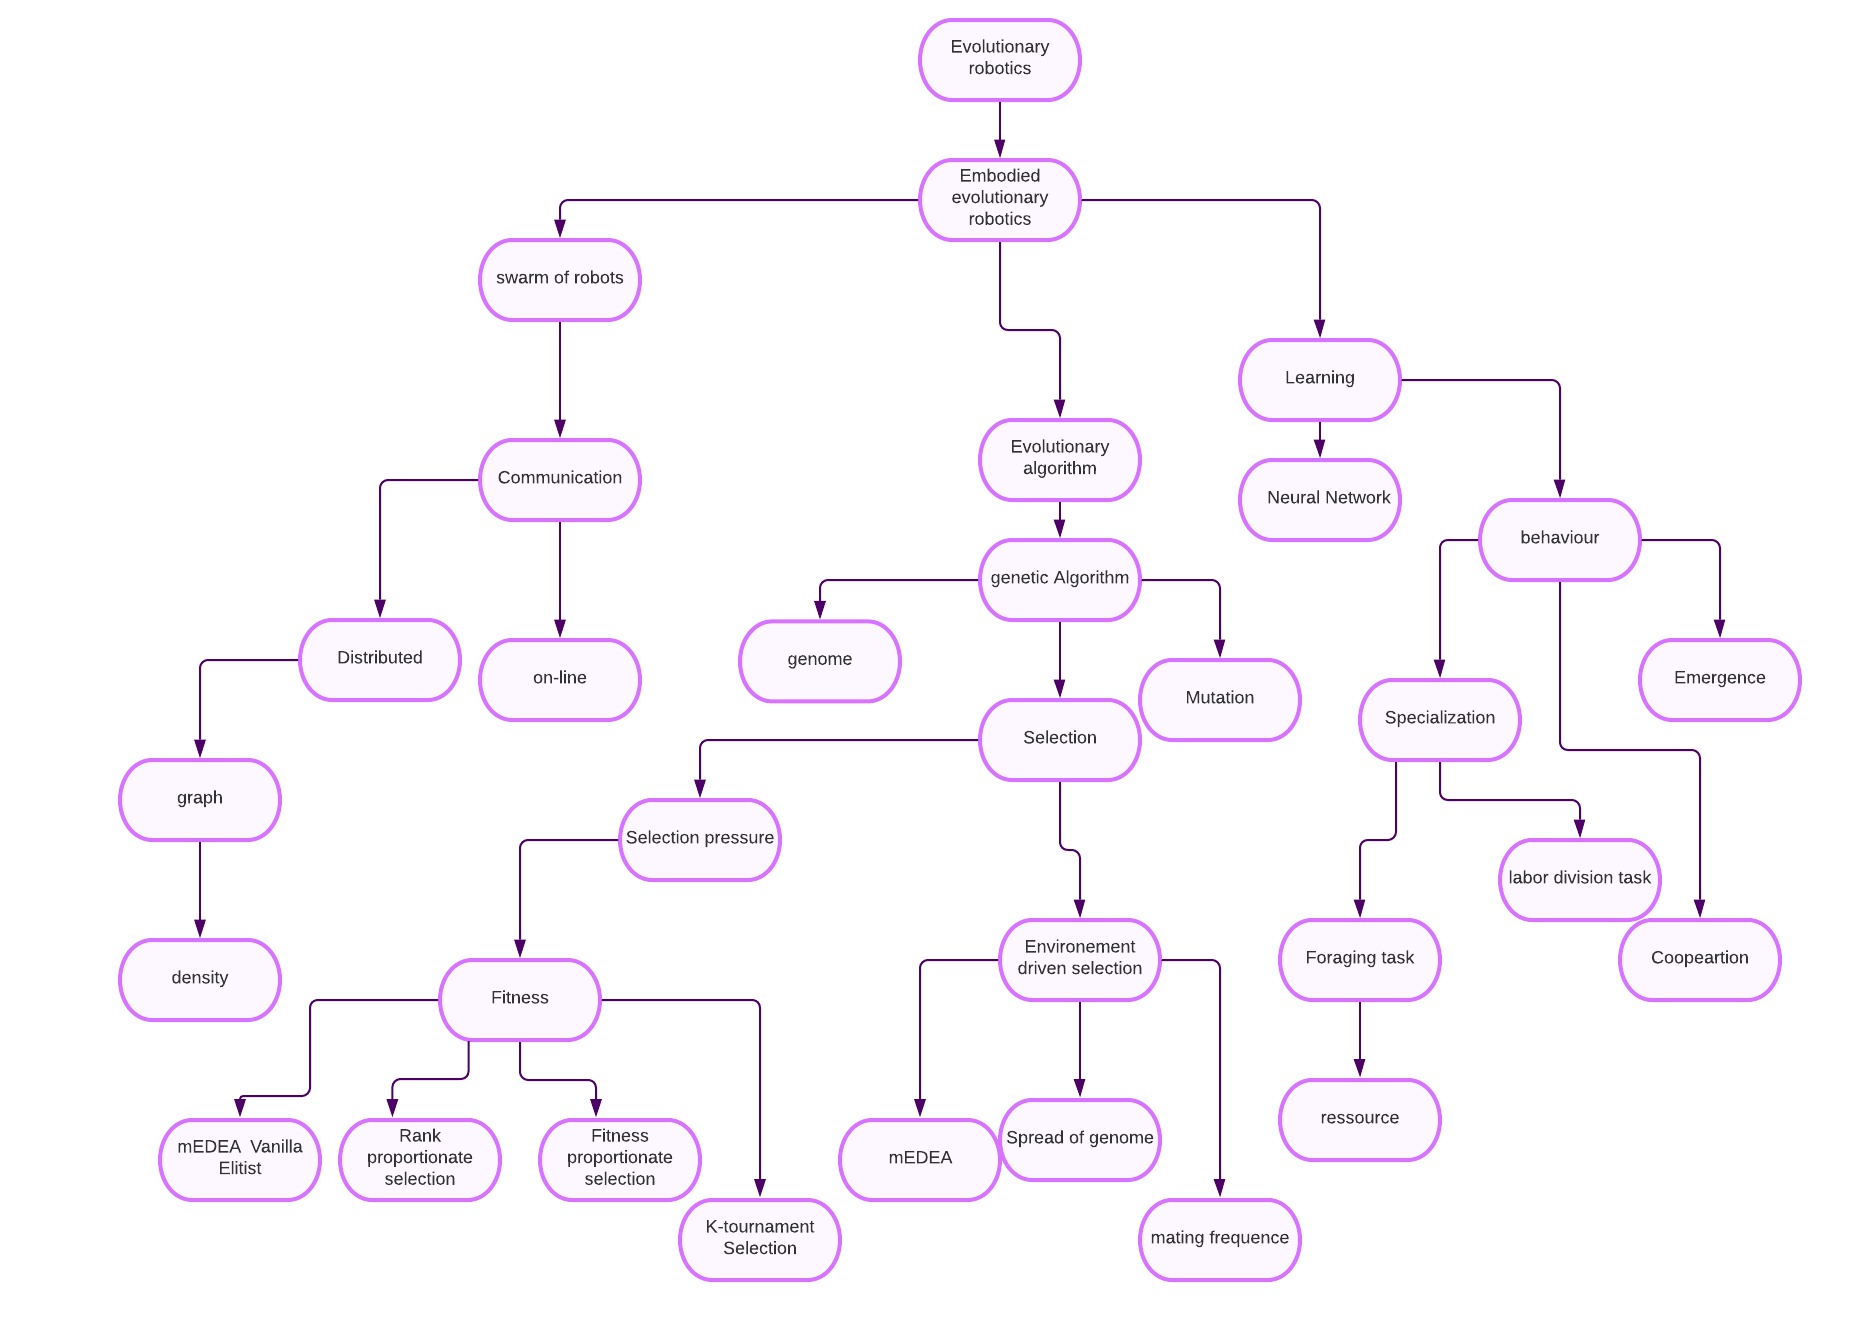
\includegraphics[scale=0.5]{carte heuristique.jpeg}

\section{Descriptif de la recherche documentaire}
On a commencé notre recherche  a partir de deux articles fournis par notre encadrant.Ils ont été publié sur « Frontiers in Robotics and AI » qui est une plateforme qui publie toutes les  théories et applications de la robotique, de la technologie et de l’intelligence artificielle, après avoir lu ces deux articles on a consulté les articles publiés dans le même thème sur cette plateforme.
   Puis on a cherché  sur Hal qui est une plateforme développé par le centre pour la communication scientifique directe destinée au dépôt et à la diffusion d’articles de recherche .Cette plateforme nous a permet d’accéder a des articles des chercheurs en utilisant les mots clés de notre projet.Ces articles nous ont fourni de nouveaux outils comme les algorithmes qui nous ont aidé à démarrer l’implémentation de notre projet.
\section{Bibliographie produite dans le cadre du projet}

\flushleft
\justify
[1]J.-M. Montanier, S. Carrignon, and N. Bredeche, “Behavioral Specialization in Embodied Evolutionary Robotics: Why So Difficult?,” Front. Robot. AI, vol. 3, 2016, doi: 10.3389/frobt.2016.00038. 
\flushleft
\justify
[2]N. Bredeche, J.-M. Montanier, and S. Carrignon, “Benefits of proportionate selection in embodied evolution: a case study with behavioural specialization,” in Proceedings of the Genetic and Evolutionary Computation Conference Companion, Berlin, Germany, Jul. 2017, pp. 1683–1684, doi: 10.1145/3067695.3082551. 

\flushleft
\justify
[3]I. F. Pérez, A. Boumaza, and F. Charpillet, “Comparison of Selection Methods in On-line Distributed Evolutionary Robotics,” presented at the The fourteenth international conference on the synthesis and simulation of living systems, Jul. 2014, doi: 10.7551/978-0-262-32621-6-ch046.

\flushleft
\justify
[4]I. F. Pérez, A. Boumaza, and F. Charpillet, “Maintaining Diversity in Robot Swarms with Distributed Embodied Evolution,” presented at the ANTS 2018 - International Conference on Swarm Intelligence, Oct. 2018, [Online]. Available: https://hal.inria.fr/hal-01937119.

\flushleft
\justify
[5]M. Brambilla, E. Ferrante, M. BIRATTARI, and M. Dorigo, “Swarm Intell Swarm robotics: a review from the swarm engineering perspective,” Swarm Intelligence, vol. 7, no. 1, pp. 1–41, 2013, doi: 10.1007/s11721-012-0075-2.

\flushleft
\justify
[6]S. van Essche, E. Ferrante, A. Turgut, R. Lon, T. Holvoet, and T. Wenseleers, “Environmental factors promoting the evolution of recruitment strategies in swarms of foraging robots,” presented at the Swarm 2015, 2015, [Online]. Available: https://hal.archives-ouvertes.fr/hal-01405907.

\flushleft
\justify
[7]I. F. Pérez, A. Boumaza, and F. Charpillet, “Influence of Selection Pressure in Online, Distributed Evolutionary Robotics,” presented at the Treizièmes Rencontres des Jeunes Chercheurs en Intelligence Artificielle (RJCIA 2015), Jun. 2015, [Online]. Available: https://hal.inria.fr/hal-01178899.

\flushleft
\justify
[8]N. Bredeche, “Embodied evolutionary robotics with large number of robots,” in 14th international conference on the synthesis and simulation of living systems (ALIFE 14), New York, United States, 2014, pp. 1–2, Accessed: Apr. 02, 2021. [Online]. Available: https://hal.archives-ouvertes.fr/hal-03175193.

\flushleft
\justify
[9]S. Doncieux, N. Bredeche, J.-B. Mouret, and A. E. (Gusz) Eiben, “Evolutionary Robotics: What, Why, and Where to,” Front. Robot. AI, vol. 2, 2015, doi: 10.3389/frobt.2015.00004.
\flushleft
\justify
[10]E. Ferrante, A. E. Turgut, E. Duéñez-Guzmán, M. Dorigo, and T. Wenseleers, “Evolution of Self-Organized Task Specialization in Robot Swarms,” PLOS Computational Biology, vol. 11, no. 8, p. e1004273, Aug. 2015, doi: 10.1371/journal.pcbi.1004273.
\flushleft
\justify

[11]I. Fernández Pérez, “Distributed Embodied Evolutionary Adaptation of Behaviors in Swarms of Robotic Agents,” Theses, Université de Lorraine, 2017.

\flushleft
\justify
[12]N. Bredeche and J.-M. Montanier, “Environment-driven Embodied Evolution in a Population of Autonomous Agents,” Sep. 2010, pp. 290–299, [Online]. Available: https://hal.inria.fr/inria-00506771.
\flushleft
\justify

[13]N. Bredeche, E. Haasdijk, and A. Prieto, “Embodied Evolution in Collective Robotics: A Review,” Front. Robot. AI, vol. 5, 2018, doi: 10.3389/frobt.2018.00012.

\section{Evaluation des ressources}
\flushleft \justify


\textbf{Behavioral Specialization in Embodied Evolutionary Robotics: Why So Difficult?:}\\
Cet article nous a été fourni par notre encadrant .Il était écrit  en 2016 par lui même , Jean-Marc Montanier et Simon Carignon qui sont tout les deux chercheurs au Computer Application in Science and Engineering (Case) a Barcelone.Ces auteurs notamment notre encadrant ont plusieurs contributions dans le domaine, ils ont publié un deuxième article une année après  la publication de cet article  dans lequel ils ont ajouté de nouvelles méthodes qui donc complètent  celui ci.\\
\textbf{Influence of Sélection Pressure in Online, Distributed Evolutionary Robotics :}\\
Cette article de conférence est écrit par Iñaki Fernández Pérez, Amine Boumaza et François Charpillet, des chercheurs à LORIA - Laboratoire Lorrain de Recherche en Informatique et ses Applications. Il a été publié à la Treizièmes Rencontres des Jeunes Chercheurs en Intelligence Artificielle (RJCIA 2015) en juin 2015.Le but de cette article était d’étudier l’impact de la pression de sélection dans l’apprentissage de stratégies collective, ce qui est donc très lié a notre projet . Dans le cadre de notre étude de l’effet de l’environnement on s’est intéressé a l’impact des différents algorithmes de sélections. On a donc réalisé une expérience similaire à celle présentée dans ce papier et nos résultats confirment bien ceux cités dans cet article. 
\textbf{Environment-driven embodied evolution in a population of autonomous agents:}\\
Cet article  écrit par Nicolas Bredeche et Jean-Marc MONTANIER qui sont des chercheurs d’ISIR(Institut des Systémes Intelligents et de Robotique ). Il a été publié  dans « Parallel Problem  Solving from Nature (PPSN) (Berlin; Heidelberg: Springer), 290–299 » en 2010 .Le but de ce papier est de proposer un nouveau algorithme efficace pour fournir une adaptation évolutive distribuée dans un environnement inconnu et résistant aux changements imprévus .
Les auteurs ont  présenté un algorithme d’adaptation  évolutionnaire qui s’appelle  MEDEA ,puis ils ont fait une analyse expérimentale approfondie de la robustesse de l’algorithme par rapport a des environnements  changeants sous des contraintes (nombre d’agents fixe).Par la suite ils ont donné  les résultats de leurs tests  .
Cet article est est très important car il nous a permet de comprendre cet algorithme qu'on a implémenté dans notre projet ,et on a eu les même résultats .On a constaté aussi que cet algorithme MEDEA est réutilisé plusieurs fois par les autres ce qui montre  la fiabilité de cet article .

\end{document}
